\documentclass{jsarticle}
\usepackage[margin = .7in]{geometry}
\usepackage[dvipdfmx]{graphicx}
\usepackage{listings}
\usepackage{amsmath}
\usepackage{bm}
\usepackage{ascmac}
\usepackage[dvipdfmx]{hyperref}
\lstset{%
  language={python},
  basicstyle={\small},%
  identifierstyle={\small},%
  commentstyle={\small\itshape},%
  keywordstyle={\small\bfseries},%
  ndkeywordstyle={\small},%
  stringstyle={\small\ttfamily},
  frame={tb},
  breaklines=true,
  columns=[l]{fullflexible},%
  numbers=left,%
  xrightmargin=0zw,%
  xleftmargin=3zw,%
  numberstyle={\scriptsize},%
  stepnumber=1,
  numbersep=1zw,%
  lineskip=-0.5ex%
}

\begin{document}
\title{卒論テーマ候補 :複数均衡}
\author{池上 慧}
\maketitle

\section{擬似データの作成}
Seim (2006)のような不完備情報の参入モデルでの複数均衡の取り扱いを調べてみました。ソースコードは\href{https://github.com/keiikegami/multiplicity}{ここ}にあります。

擬似データとして、以下のようなデータを作成するコードを書きました。
\begin{center}
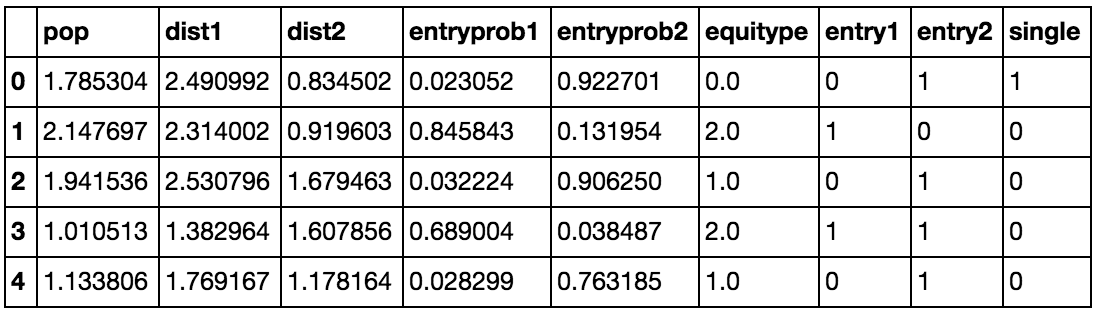
\includegraphics[width=10cm]{table1.png}
\end{center}
データの作成に関してのnotebookは\href{https://github.com/keiikegami/multiplicity/blob/master/sample_data_generation.ipynb}{こちら}にあります。

ここで行はサンプルとして得られている市場を、popは人口、dist1が企業1のコストを、dist2が企業2のコスト、entryprobはそれぞれの市場でモデルの均衡が与える参入確率のうち選択されたもの、equitypeは0が一つしか均衡がないことを1が複数均衡が存在した時に安定的な均衡のうちの片方が選ばれたこと、2はその逆の均衡が選ばれたことをそれぞれ示しています。singleは一つしかモデルに均衡が存在しないことを示すダミー変数です。結果として各企業が参入したか否かはentry1とentry2でダミー変数として表示されています。

このモデルでは、$\sigma_{-i}^j$を市場$j$における$i$じゃない方の企業の参入確率として、市場$j$における企業$i$の利得関数以下のように特定している。
\begin{align}
	u_i^j = \alpha\ pop_j + \beta\ dist_i^j + \delta\  \sigma_{-i}^{j} + \epsilon_i^j
\end{align}

なのでパラメータは$(\alpha, \beta, \delta)$の3つである。また、popは正の実数のみをサポートに持つlocation 1の打ち切り正規分布、distは$(1.2, 0.8)$をlocationとして持つ、正の実数のみをサポート荷物打ち切り2変量正規分布で発生させている。

この変数に対してモデルが複数の均衡を出すこともあれば単一の均衡を出すこともあるようなパラメータとして、以下の4つのパラメータセットを提示する。均衡がどのように出るかを可視化したnote bookは\href{https://github.com/keiikegami/multiplicity/blob/master/best_response_function.ipynb}{こちら}。
\begin{description}
	\item[Param1] $\alpha = 1.7, \beta = -0.5, \delta = -6$
	\item[Param2] $\alpha = 1.7, \beta = -4.5, \delta = -6$
	\item[Param3] $\alpha = 1.7, \beta = -0.5, \delta = 6$
	\item[Param4] $\alpha = 1.7, \beta = -4.5, \delta = 6$
\end{description}
擬似データの作成は先の4つの代表的なパラメータセットを始め、任意のパラメータ、任意の変数の大きさに対して出力できるように作られている。また、複数の均衡があった場合には安定的な均衡はこのモデルでは通常2つ存在し、その選ばれる確率も一つのパラメータとして設定することができる。

\section{やってみたこと}
\subsection{均衡の種類の分類}
データドリブンな手法を用いて均衡の種類を分類できないかを試してみた。note bookは\href{https://github.com/keiikegami/multiplicity/blob/master/prediction2.ipynb}{こちら}。

単純なk-meansで分類してみると、先のパラメータセットで1は比較的よく分類できた。すなわち各市場でどの均衡が実現しているかをある程度分類できている。この時は、クラスター数を2つで分類した結果とクラスター数を3つで分類した結果を合わせることで各市場が単一均衡なのか、複数均衡なのかを一定の精度で見分けることができる。しかし他のパラメータセットでは分類がうまく分類できない。

このようなパラメータによる分類結果の差がどのような理由によるのかはまだ考えていない。しかしもしうまく分類できるのなら、実際に推定する際に均衡が複数存在する市場として扱わなくてはならない市場と、そうではない市場とを区別することができる。

\subsection{単一均衡の仮定による影響}
Seim (2006)などをはじめとして不完備情報の参入退出モデルの推定には、単一均衡の仮定に基づいた二段階推定がよく用いられる。ここで「単一均衡の仮定」とは、この手法で推定されたパラメータの値に対してモデルが複数の均衡を出す場合でも、実際に観測された均衡でない方の均衡が実現する確率は0である、という仮定である。

この過程の妥当性を評価するために、先の擬似データを用いて、本来の参入確率とノンパラメトリックな手法によって予測される参入確率とを散布図でプロットしてみた。































\end{document}
